\documentclass[12pt,addpoints]{exam}
%\usepackage{dsfont}
\usepackage{amsfonts}
\usepackage{amsmath}
\usepackage{array}
\usepackage{tabularx}
\usepackage{etoolbox}
\usepackage{eso-pic}


\usepackage[letterpaper,top=1.55cm, bottom=3.5cm, outer=4cm, inner=3cm,
heightrounded, marginparwidth=0cm,marginparsep=1cm]{geometry}

\newtoggle{compress}
\toggletrue{compress}
% \togglefalse{compress}


\usepackage{color}

\usepackage{graphicx}
%% \usepackage{geometry}
\usepackage{color}
\usepackage{hyperref}
\hypersetup{
  pdftitle={Limits worksheet},
  pdfsubject={Calculus},
  pdfauthor={Kelly Black},
  pdfkeywords={limits},
  anchorcolor = {red},
  colorlinks = {true},
  runcolor = {black},
  linkcolor = {black},
  urlcolor = {black},
  %% pdfpagemode={FullScreen}
}


\usepackage{tikz}
\usepackage{pgf}
\usepackage{pgfplots}
\usepgfplotslibrary{fillbetween}
% \pgfplotsset{width=7cm}
\usepgfplotslibrary{patchplots}


%% \oddsidemargin=-0.5in
%% \evensidemargin=-0.5in
%% \textwidth=6.5in

%% \topmargin=-0.75in
%% \textheight=9.5in

\pagestyle{plain}
\reversemarginpar

%%%%%%%%%%%%%%%%%%%%%%%%%%%%%%%%%%%%%%%%%%%%%%%%%%%%%%%%%%%%%%%%%%%
%%%%%%%%%%%%%%%%%%%%%%%%%%%%%%%%%%%%%%%%%%%%%%%%%%%%%%%%%%%%%%%%%%%
 \def\Course{Math 1113}
 \def\NumSec{23879}
 \def\time{10:10am-11:00am}
 \def\Date{Friday, 1 Feb 2019}
 \def\test{In Class}
 \def\version{A}
%%%%%%%%%%%%%%%%%%%%%%%%%%%%%%%%%%%%%%%%%%%%%%%%%%%%%%%%%%%%%%%%%%%
%%%%%%%%%%%%%%%%%%%%%%%%%%%%%%%%%%%%%%%%%%%%%%%%%%%%%%%%%%%%%%%%%%%
 \pagestyle{headandfoot}
 \headrule
 \firstpageheader{\bf University of Georgia \\
                    Department of Mathematics               \\
                  \Date}
                 {\bf\Course\ --- \NumSec
                  \\ \test \\[-5pt] \ }
                 {\bf Name:\enspace\hbox to 2in{\hrulefill} \\
                  {\tiny(BLOCK/CAPITAL LETTER)}\hspace{0.75cm}\,}
  \runningheadrule
  \runningheader{\Course}{\test, Section \NumSec}{\Date}
  \footrule
  \firstpagefooter{[\version]}
  {Page \thepage\ of \numpages}
  {\rule{0cm}{.35cm} }
  \runningfooter  {[\version]}
  {Page \thepage\ of \numpages}
  {\rule{0cm}{.35cm} }
%%%%%%%%%%%%%%%%%%%%%%%%%%%%%%%%%%%%%%%%%%%%%%%%%%%%%%%%%%%%%%%%%%%
 \extrawidth     { 1.00in}
 \extraheadheight{0.15in}%[-0.30in]{-0.30in}
 \extrafootheight{0.21in}
 \addpoints
 %%%%%%%%%%%%%%%%%%%%%%%%%%%%%%%%%%%%%%%%%%%%%%%%%%%%%%%%%%%%%%%%%%%




\begin{document}

%% <%include file="coverPage.template"/>

Complete Before Class:
\begin{questions}
\question 
  Three  equations are defined by
  \begin{eqnarray*}
    \mathrm{Avril(x)} & = & x^2, \\
    \mathrm{Arnold(x)} & = & x, \\
    \mathrm{Angus(x)} & = & 1.
  \end{eqnarray*}


  \begin{parts}
  \part Write out the function
    \begin{eqnarray*}
      8*\mathrm{Avril}(x) - 3*\mathrm{Arnold}(x) + 10*\mathrm{Angus}(x)
    \end{eqnarray*}
    as a quadratic polynomial.

    \vfill
    
    \part A function is defined by
  \begin{eqnarray*}
    \mathrm{Amy}(x) & = & 3 x^2 + 2x +5.
  \end{eqnarray*}
  Express the function Amy in terms of Avril, Arnold, and Angus.

  \vfill
  
  \end{parts}
\end{questions}


\clearpage

\begin{questions}


 \question Given the two functions defined below provide formulas for
   the expressions below:
   \begin{eqnarray*}
     \mathrm{Axel(x)} & = & x + 5, \\
     \mathrm{Ava(x)} & = & \sqrt{x}.
   \end{eqnarray*}
  \begin{parts}
    \part  ${\displaystyle \left( \mathrm{Axel}+\mathrm{Ava}\right)(x) } $
    
      \vfill

    \part  ${\displaystyle \left( 3\mathrm{Axel}-\mathrm{Ava}\right)(x) } $
    
    %% <%include file="questionResults.template"/>    

      \vfill

    \part  ${\displaystyle \left( \mathrm{Axel} \cdot \mathrm{Ava}\right)(x)  }$
    
    %% <%include file="questionResults.template"/>    

      \vfill    

    \part  ${\displaystyle \left( \mathrm{Axel} \div \mathrm{Ava}\right)(x)  }$
    
    %% <%include file="questionResults.template"/>    

      \vfill    

\end{parts}


\clearpage

 \question Given the two functions defined below provide formulas for
   the expressions below:
   \begin{eqnarray*}
     \mathrm{Axel(x)} & = & x + 5, \\
     \mathrm{Ava(x)} & = & \sqrt{x}.
   \end{eqnarray*}
  \begin{parts}
  \part  ${\displaystyle \frac{\mathrm{Axel}(x+2)-\mathrm{Axel}(x)}{2} } $
    (Simplify your expression as much as possible.)
    
    \vfill

  \part  ${\displaystyle \frac{\mathrm{Ava}(x+2)-\mathrm{Ava}(x)}{2} } $
    (Simplify your expression as much as possible.)
    
    \vfill

  \part  ${\displaystyle \mathrm{Axel}\left(\mathrm{Ava}(x)\right) } $
    
    \vfill

\end{parts}


\clearpage



\question Information about two functions, $\mathrm{Abbot}$ and $\mathrm{Costello}$, 
  is given below. Use the information to answer the questions that
  follow.

    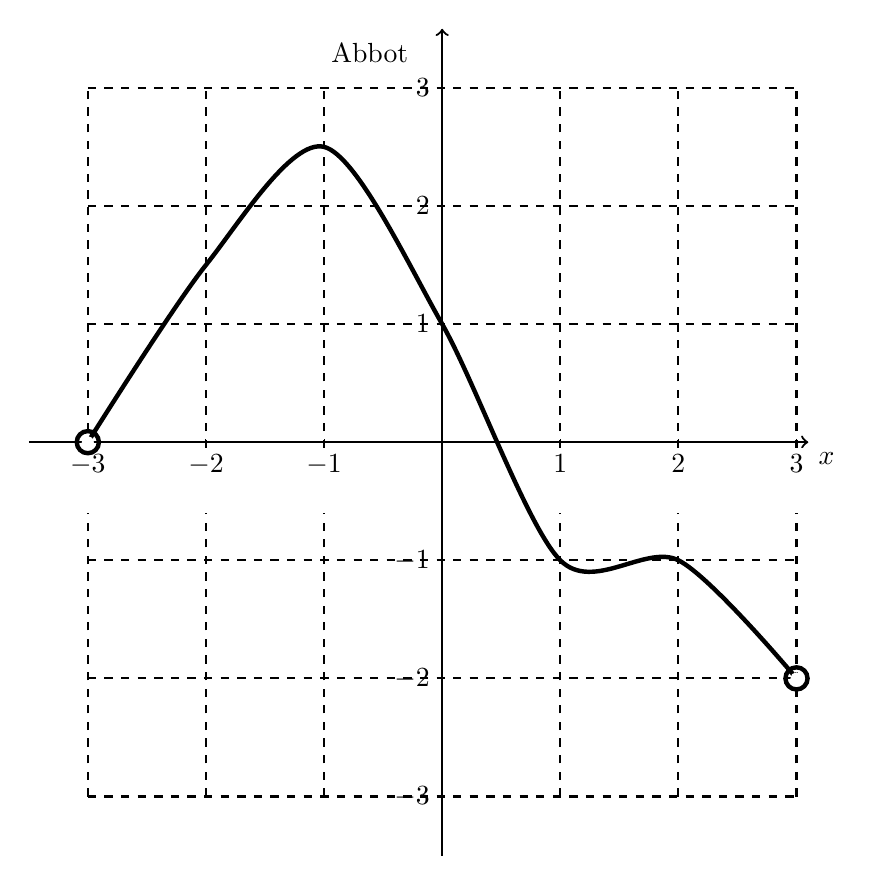
\begin{tikzpicture}[y=1.5cm, x=1.5cm,font=\sffamily]
      \begin{scope}[shift={(0,0)}]
        % ticks
        \draw[xstep = 1,ystep=1,black,dashed,thick] % very thin,opacity=0.85,
        (-3.0, -3.0) grid ( 3.0, 3.0);
        % axis
        \draw[thick,->] (-3.5,0) -- coordinate (x axis mid) (3.1,0)
        node[anchor = north west] {$x$};

        \draw[thick,->] (0,-3.5) -- coordinate (y axis mid) (0,3.5)
        node[anchor = east,shift={(-0.2,-0.2)}] {{$\mathrm{Abbot}$}};

        \foreach \y in {-3,-2,-1,1,2,3} { 
          \draw (1pt, \y) -- (-1pt,\y) node[anchor = east] {$\y$}; 
        }

        \foreach \x in {-3,-2,-1,1,2,3} { 
          \fill[white] (\x-0.1,-0.6) rectangle (\x+0.1,-0.05); 
          \draw (\x,1pt) -- (\x,-1pt) node[anchor =north] {$\x$}; 
        }

        \draw[ultra thick] plot [smooth] coordinates {(-3,0) (-2,1.5)(-1,2.5) (0,1)(1,-1)(2,-1)(3,-2) };
        \draw[ultra thick] (-3,0) circle (4pt);
        \filldraw[color=white] (-3,0) circle (2pt);
        \draw[ultra thick] (3,-2) circle (4pt);
        \filldraw[color=white] (3,-2) circle (2pt);
      \end{scope}
    \end{tikzpicture}

    \begin{eqnarray*}
      \mathrm{Costello}(x) & = &
                                 \left\{
                                 \begin{array}{l@{\hspace{3em}}rcccl}
                                   2x  & -2 & \leq & x & < & 0, \\
                                   1-x & 0 & \leq & x & < & 2.
                                 \end{array}
                                 \right.
    \end{eqnarray*}

\begin{parts}

\part  Determine the value of ${\displaystyle \mathrm{Costello}\left(\mathrm{Abbot}(1)\right) }$.
  
  \vfill

\part  Determine the value of ${\displaystyle \mathrm{Abbot}\left(\mathrm{Costello}(1)\right) }$.
  
  \vfill

\part  Determine the value of ${\displaystyle \mathrm{Costello}\left(\mathrm{Abbot}(-1)\right) }$.
  
  \vfill

\end{parts}




\end{questions}


\end{document}

